\appendix{Представление графического материала}

Графический материал, выполненный на отдельных листах,
изображен на рисунках А.1--А.\arabic{числоПлакатов}.
\setcounter{числоПлакатов}{0}

\renewcommand{\thefigure}{А.\arabic{figure}} % шаблон номера для плакатов

\begin{плакат}
    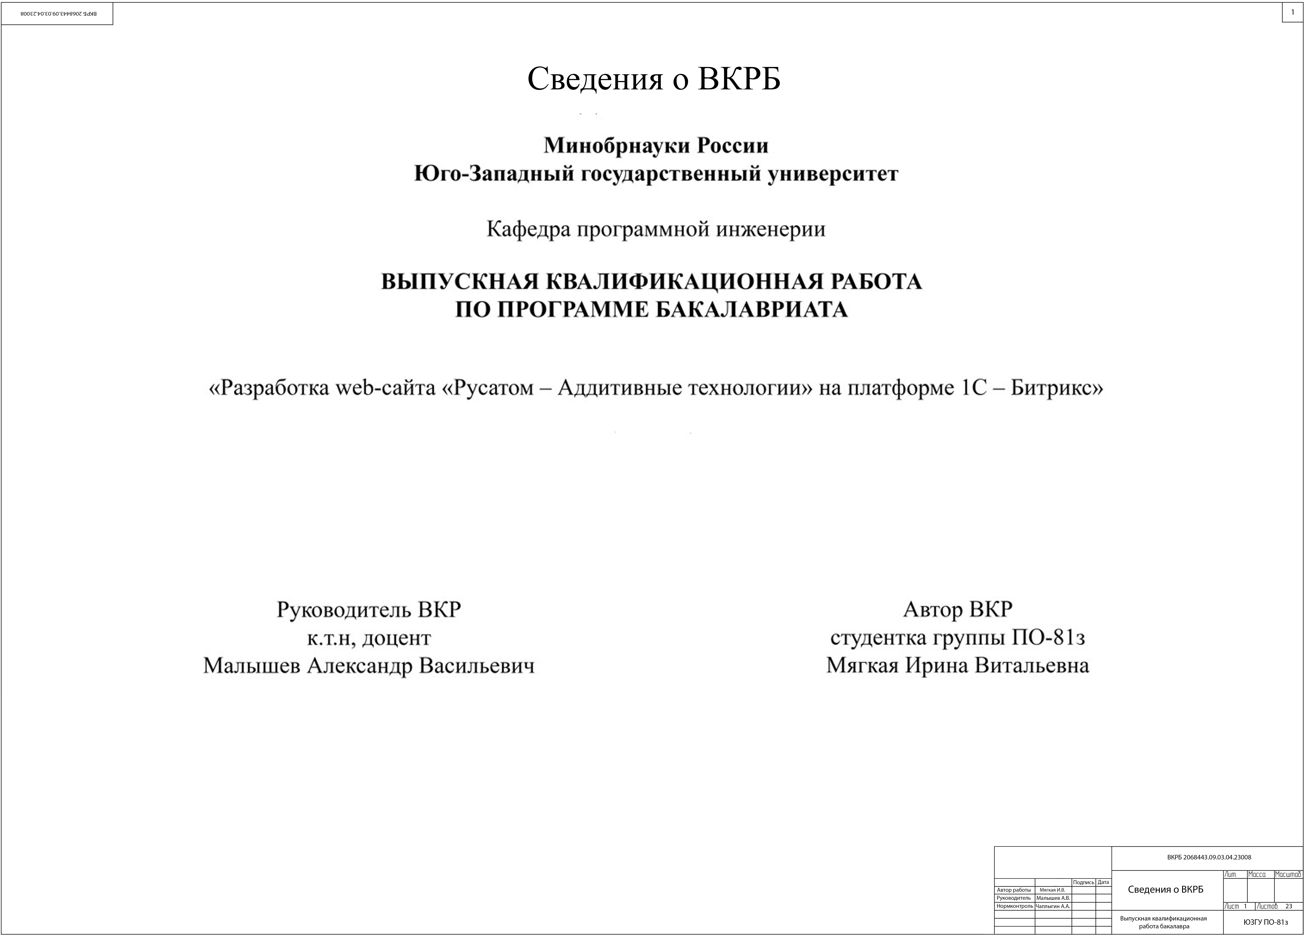
\includegraphics[width=1\linewidth]{плакат1.png}
    \заголовок{Сведения о ВКРБ}
    \label{pl1:image}      
\end{плакат}

\begin{плакат}
    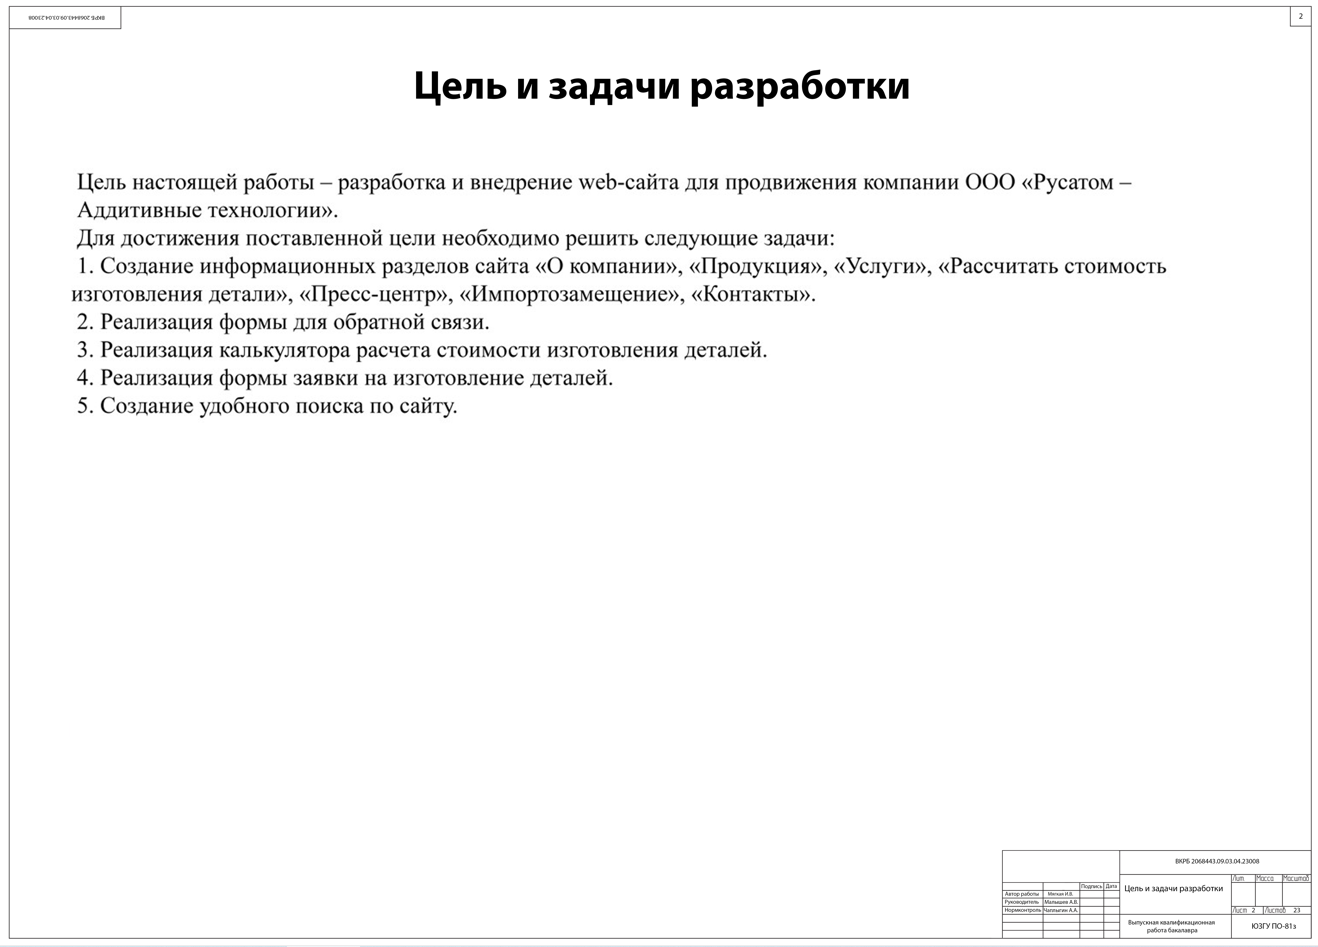
\includegraphics[width=1\linewidth]{плакат2.png}
    \заголовок{Цель и задачи разработки}
    \label{pl2:image}      
\end{плакат}

\begin{плакат}
    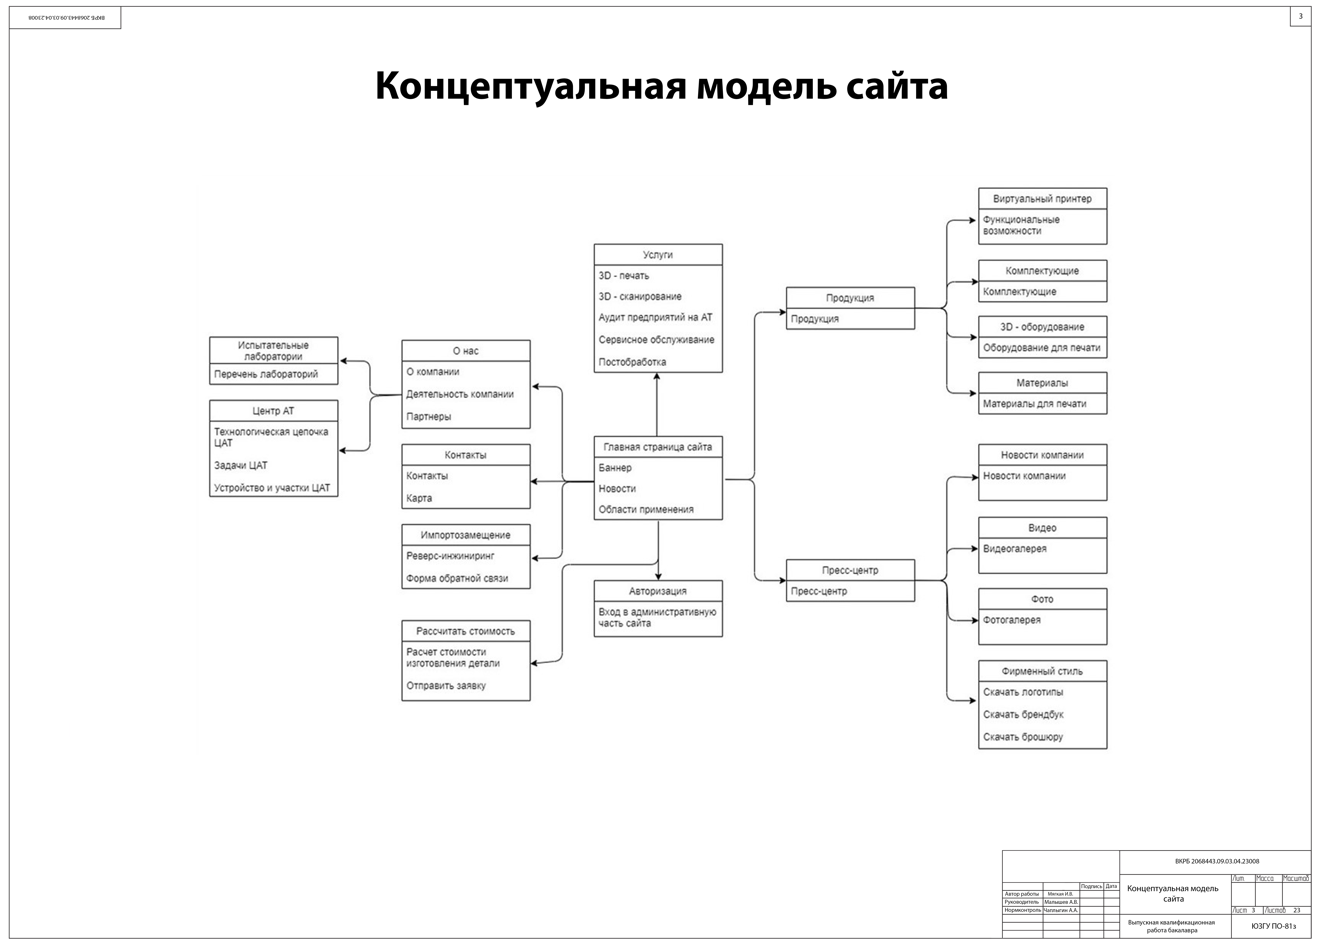
\includegraphics[width=1\linewidth]{плакат3.png}
    \заголовок{Концептуальная модель сайта}
    \label{pl3:image}      
\end{плакат}

\begin{плакат}
    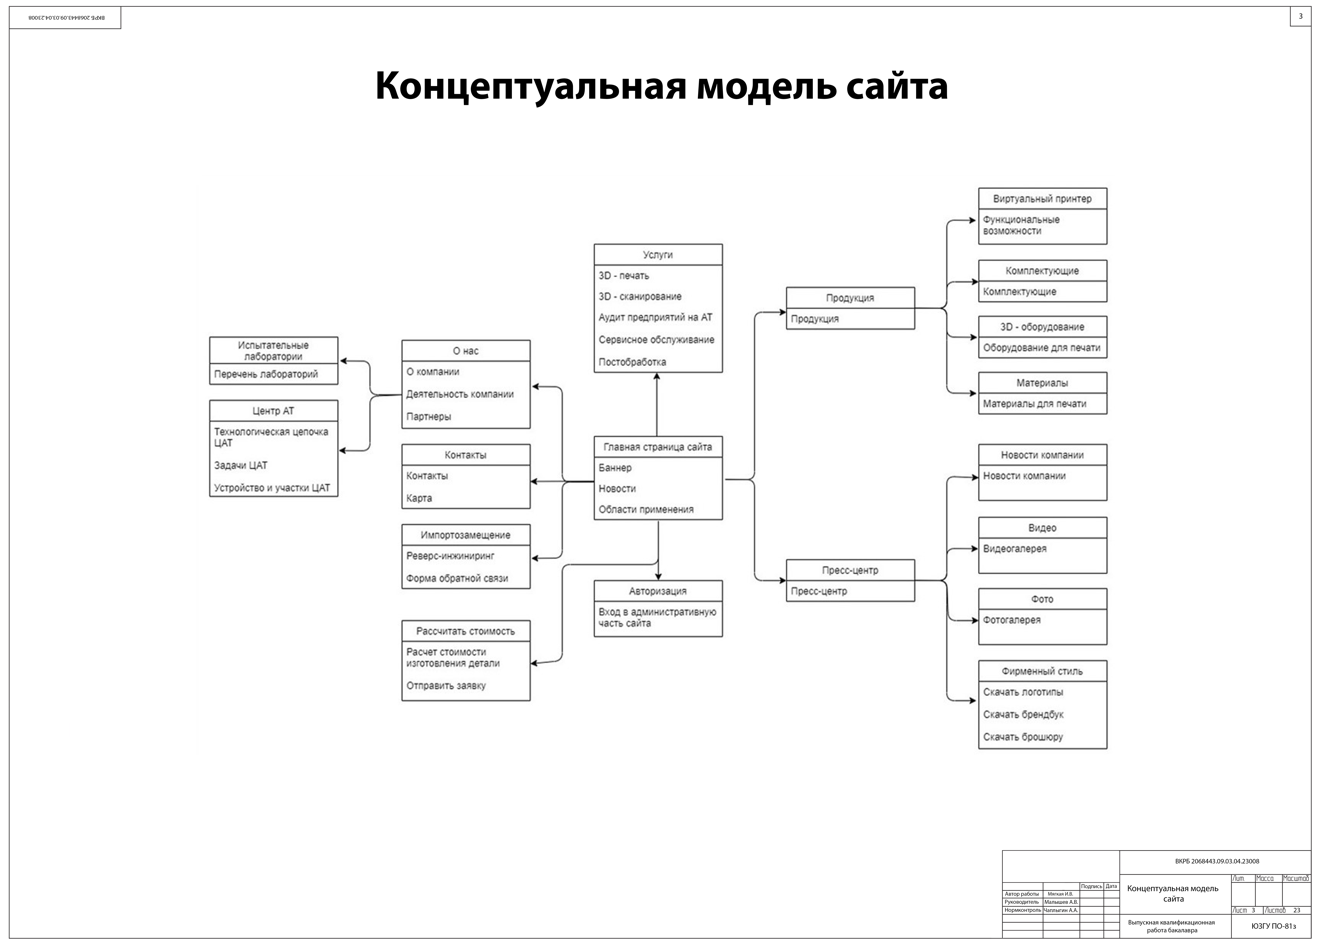
\includegraphics[width=1\linewidth]{плакат3.png}
    \заголовок{Еще плакат}
    \label{pl4:image}      
\end{плакат}

%\begin{figure}
%  \begin{adjustbox}{addcode={\begin{minipage}{\width}}{\caption{%
%          Сведения о ВКРБ
%      }\end{minipage}},rotate=90,center}
%    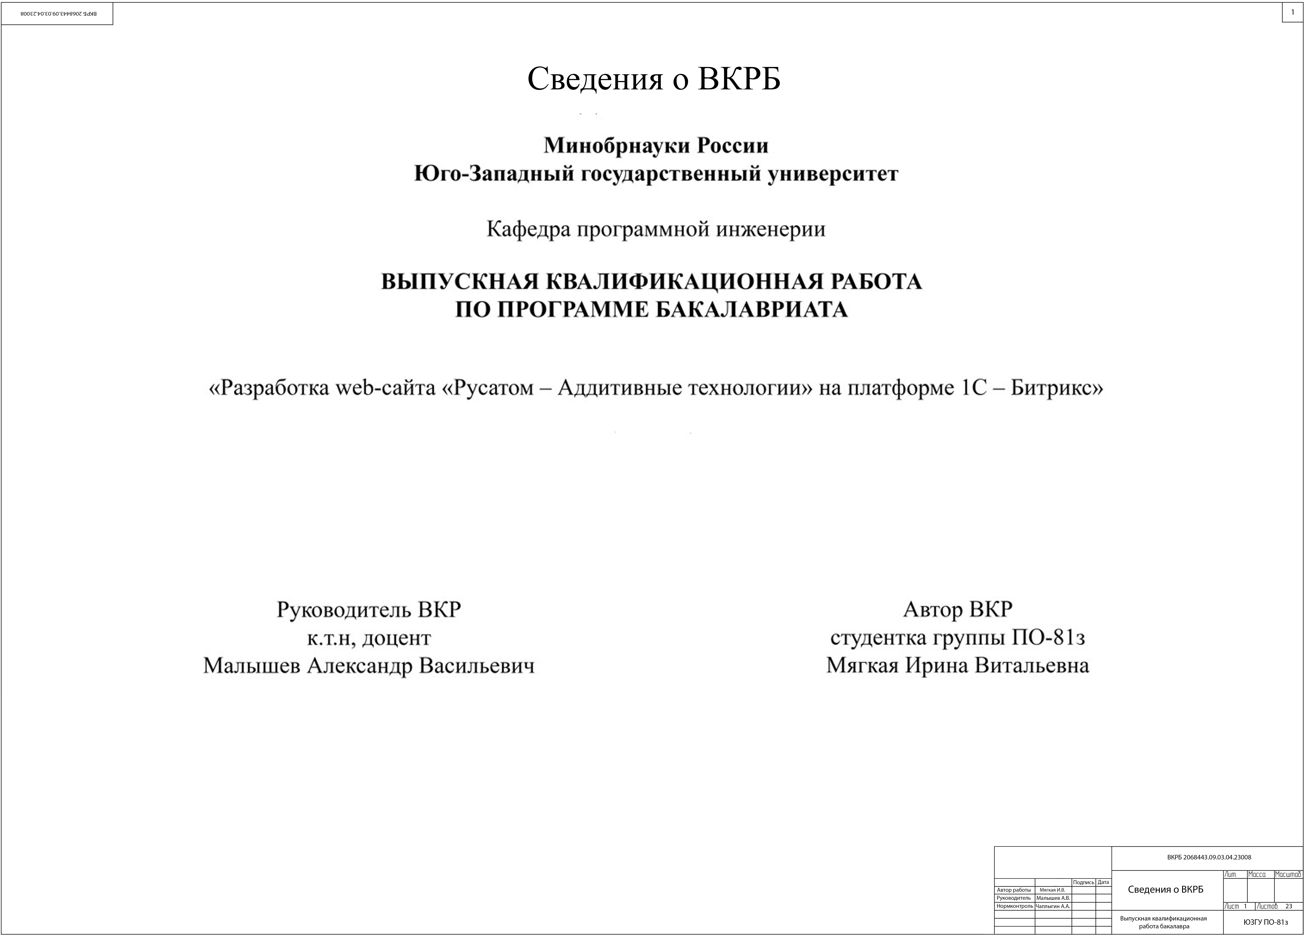
\includegraphics[width=1.3\linewidth]{плакат1.png}
%  \end{adjustbox}
%  \label{pl1:image}      
%\end{figure}

%\begin{figure}
%  \begin{adjustbox}{addcode={\begin{minipage}{\width}}{\caption{%
%          Цель и задачи разработки
%      }\end{minipage}},rotate=90,center}
%    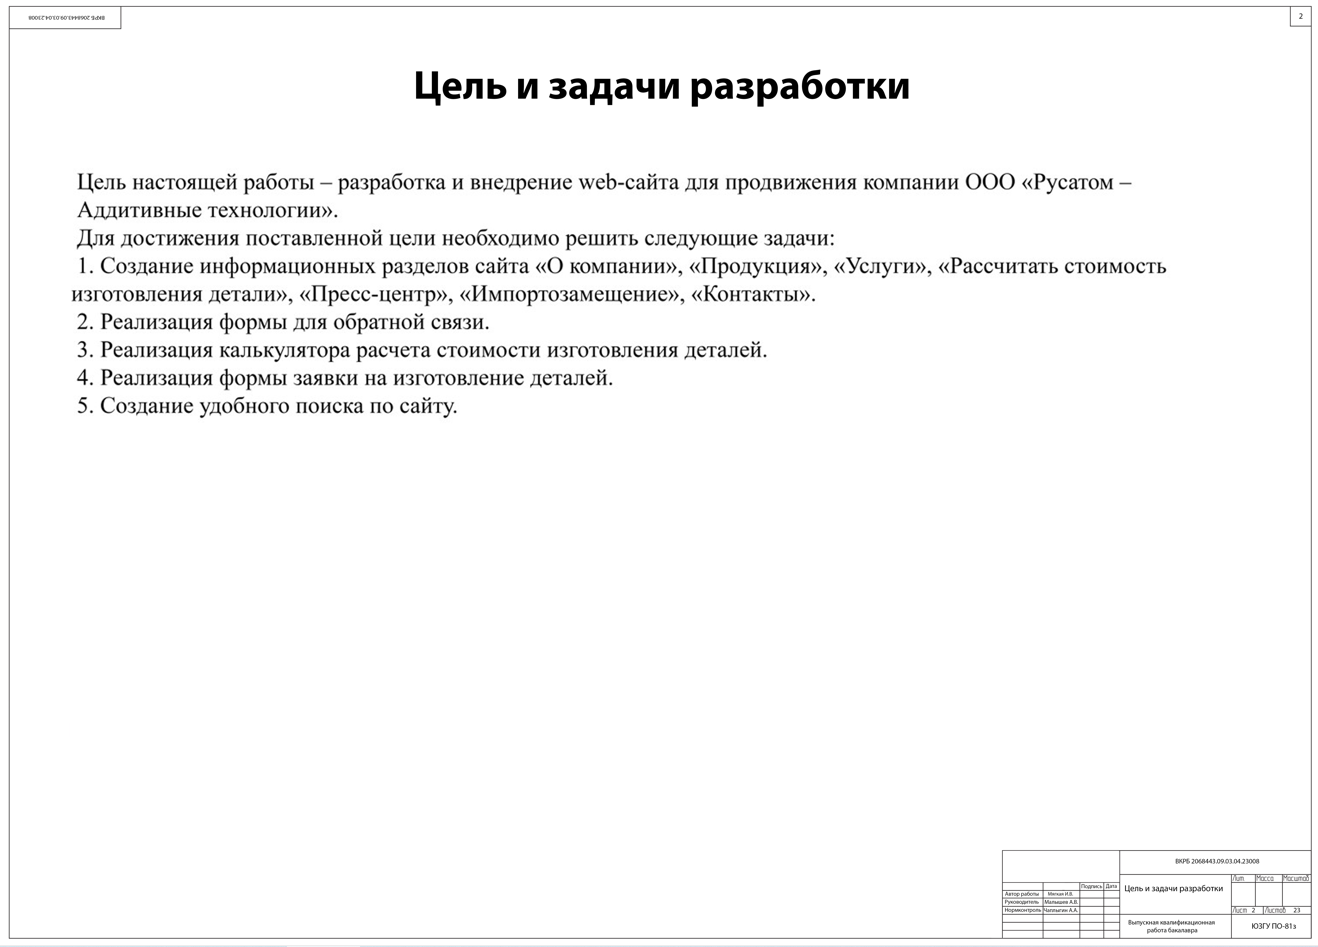
\includegraphics[width=1.3\linewidth]{плакат2.png}
%  \end{adjustbox}
%  \label{pl2:image}      
%\end{figure}

%\begin{figure}
%  \begin{adjustbox}{addcode={\begin{minipage}{\width}}{\caption{%
%          Концептуальная модель сайта
%      }\end{minipage}},rotate=90,center}
%    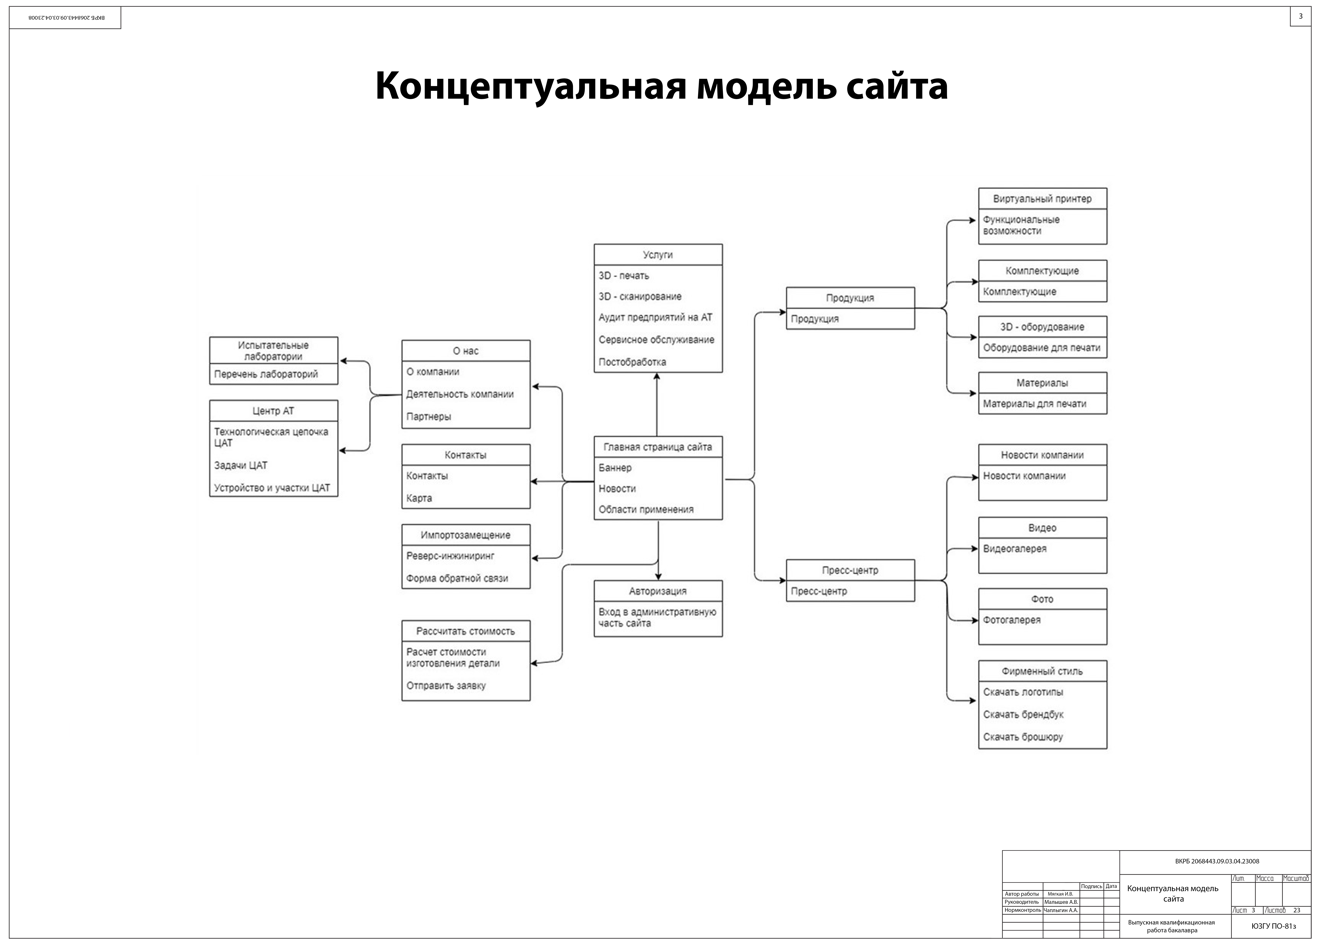
\includegraphics[width=1.3\linewidth]{плакат3.png}
%  \end{adjustbox}
%  \label{pl3:image}      
%\end{figure}
